\documentclass[tikz,border=2pt]{standalone}
\usepackage{newpxtext,newpxmath}
\definecolor{curve}{HTML}{1f6fb2}
\definecolor{accent}{HTML}{c0392b}
\definecolor{polygon}{HTML}{555555}
\definecolor{muted}{HTML}{dfe6ee}
\begin{document}
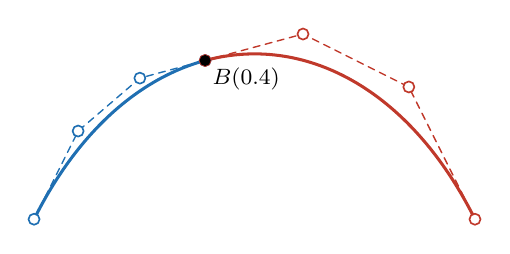
\begin{tikzpicture}[
  x=1.4cm, y=1.4cm,
  line cap=round, line join=round,
  every node/.style={font=\footnotesize, inner sep=1.5pt},
  curve/.style={draw=curve, line width=1.1pt},
  second/.style={draw=accent, line width=1.1pt},
  polygon/.style={line width=0.5pt, dash pattern=on 2.5pt off 2pt},
  construction/.style={draw=accent, line width=0.5pt},
  axis/.style={line width=0.45pt, draw=black!80, >=stealth},
  ctrl/.style={circle, fill=white, line width=0.6pt, minimum size=4pt, inner sep=0pt},
]
\draw[curve] (0.0000,0.0000) .. controls (0.4000,0.8000) and (0.9600,1.2800) .. (1.5520,1.4400);
\draw[second] (1.5520,1.4400) .. controls (2.4400,1.6800) and (3.4000,1.2000) .. (4.0000,0.0000);
\draw[polygon, draw=curve] (0,0) -- (0.4,0.8) -- (0.96,1.28) -- (1.552,1.44);
\node[ctrl, draw=curve] at (0,0) {};
\node[ctrl, draw=curve] at (0.4,0.8) {};
\node[ctrl, draw=curve] at (0.96,1.28) {};
\node[ctrl, draw=curve] at (1.552,1.44) {};
\draw[polygon, draw=accent] (1.552,1.44) -- (2.44,1.68) -- (3.4,1.2) -- (4,0);
\node[ctrl, draw=accent] at (1.552,1.44) {};
\node[ctrl, draw=accent] at (2.44,1.68) {};
\node[ctrl, draw=accent] at (3.4,1.2) {};
\node[ctrl, draw=accent] at (4,0) {};
\fill[black] (1.552,1.44) circle (2pt);
\node[below right=1pt] at (1.552,1.44) {$B(0.4)$};
\end{tikzpicture}
\end{document}
